\documentclass[../SpecificaTecnica.tex]{subfiles}
\begin{document}
	\section{Joint}
La libreria JointJS è una libreria open source per diagrammi scritta in JavaScript e sviluppata
da clientIO (client.io).
Le principali funzionalit\'a ed elementi fornite dalla libreria che vengono sfruttate nel programma sono:
\begin{itemize}
\item elementi per diagrammi base (e.g. rettangoli, cerchi, testo, immagini);
\item diagrammi già pronti all’uso;
\item elementi custom basati su SVG;
\item elementi (Elements) e collegamenti (Link) interattivi;
\item collegamenti personalizzabili (punta, etichette);
\item elementi magnetici;
\item diagrammi gerarchici;
\item altamente event-driven;
\item zoom in/out.
\end{itemize}

\begin{figure}[H] \label{fig:Joint}
	\centering
	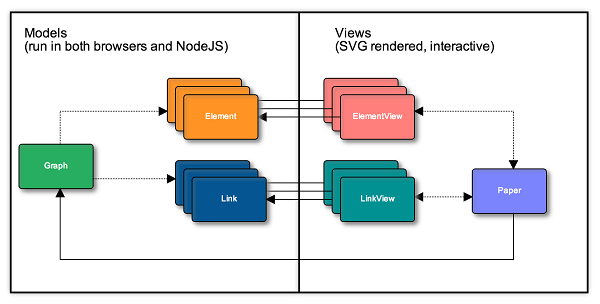
\includegraphics[scale=1]{Immagini/joint.png}
	\caption{Schema Joint}
\end{figure}

La figura precedente mostra un'esemplificazione del funzionamento di Joint.\\
La creazione di un nuovo diagramma è piuttosto semplice: è sufficiente specificare un Graph sul quale un Paper deve rimanere in ascolto (observe).\\
È possibile catturare eventi all’interno del Paper e gestirli di conseguenza.\\
Il Graph possiede al suo interno una GraphCells. Questa rappresenta il raccoglitore di celle (Cell, che costituiscono gli elementi da cui è composto un Graph.\\
Una Cell è osservata da una CellView del tutto simile in funzionamento a quanto accade tra un model ed una view.
Ereditando da Cell (o meglio, dalle appropriate sottoclassi) possiamo disporre già di svariati metodi già implementati e testati da JointJS.

\end{document}